% Options for packages loaded elsewhere
\PassOptionsToPackage{unicode}{hyperref}
\PassOptionsToPackage{hyphens}{url}
%
\documentclass[
  ignorenonframetext,
]{beamer}
\usepackage{pgfpages}
\setbeamertemplate{caption}[numbered]
\setbeamertemplate{caption label separator}{: }
\setbeamercolor{caption name}{fg=normal text.fg}
\beamertemplatenavigationsymbolsempty
% Prevent slide breaks in the middle of a paragraph
\widowpenalties 1 10000
\raggedbottom
\setbeamertemplate{part page}{
  \centering
  \begin{beamercolorbox}[sep=16pt,center]{part title}
    \usebeamerfont{part title}\insertpart\par
  \end{beamercolorbox}
}
\setbeamertemplate{section page}{
  \centering
  \begin{beamercolorbox}[sep=12pt,center]{part title}
    \usebeamerfont{section title}\insertsection\par
  \end{beamercolorbox}
}
\setbeamertemplate{subsection page}{
  \centering
  \begin{beamercolorbox}[sep=8pt,center]{part title}
    \usebeamerfont{subsection title}\insertsubsection\par
  \end{beamercolorbox}
}
\AtBeginPart{
  \frame{\partpage}
}
\AtBeginSection{
  \ifbibliography
  \else
    \frame{\sectionpage}
  \fi
}
\AtBeginSubsection{
  \frame{\subsectionpage}
}
\usepackage{lmodern}
\usepackage{amssymb,amsmath}
\usepackage{ifxetex,ifluatex}
\ifnum 0\ifxetex 1\fi\ifluatex 1\fi=0 % if pdftex
  \usepackage[T1]{fontenc}
  \usepackage[utf8]{inputenc}
  \usepackage{textcomp} % provide euro and other symbols
\else % if luatex or xetex
  \usepackage{unicode-math}
  \defaultfontfeatures{Scale=MatchLowercase}
  \defaultfontfeatures[\rmfamily]{Ligatures=TeX,Scale=1}
\fi
% Use upquote if available, for straight quotes in verbatim environments
\IfFileExists{upquote.sty}{\usepackage{upquote}}{}
\IfFileExists{microtype.sty}{% use microtype if available
  \usepackage[]{microtype}
  \UseMicrotypeSet[protrusion]{basicmath} % disable protrusion for tt fonts
}{}
\makeatletter
\@ifundefined{KOMAClassName}{% if non-KOMA class
  \IfFileExists{parskip.sty}{%
    \usepackage{parskip}
  }{% else
    \setlength{\parindent}{0pt}
    \setlength{\parskip}{6pt plus 2pt minus 1pt}}
}{% if KOMA class
  \KOMAoptions{parskip=half}}
\makeatother
\usepackage{xcolor}
\IfFileExists{xurl.sty}{\usepackage{xurl}}{} % add URL line breaks if available
\IfFileExists{bookmark.sty}{\usepackage{bookmark}}{\usepackage{hyperref}}
\hypersetup{
  pdftitle={Charitable Giving, Tax Reform, and Political Trust},
  pdfauthor={Hiroki Kato\^{}1; Tsuyoshi Goto\^{}2; Yong-Rok Kim\^{}3},
  hidelinks,
  pdfcreator={LaTeX via pandoc}}
\urlstyle{same} % disable monospaced font for URLs
\newif\ifbibliography
\usepackage{graphicx}
\makeatletter
\def\maxwidth{\ifdim\Gin@nat@width>\linewidth\linewidth\else\Gin@nat@width\fi}
\def\maxheight{\ifdim\Gin@nat@height>\textheight\textheight\else\Gin@nat@height\fi}
\makeatother
% Scale images if necessary, so that they will not overflow the page
% margins by default, and it is still possible to overwrite the defaults
% using explicit options in \includegraphics[width, height, ...]{}
\setkeys{Gin}{width=\maxwidth,height=\maxheight,keepaspectratio}
% Set default figure placement to htbp
\makeatletter
\def\fps@figure{htbp}
\makeatother
\setlength{\emergencystretch}{3em} % prevent overfull lines
\providecommand{\tightlist}{%
  \setlength{\itemsep}{0pt}\setlength{\parskip}{0pt}}
\setcounter{secnumdepth}{-\maxdimen} % remove section numbering
\setbeamertemplate{navigation symbols}{}
\setbeamertemplate{footline}[page number]

\usepackage{bookmark}
\usepackage{booktabs}

\usepackage{xltxtra} 
\usepackage{zxjatype} 
\usepackage[ipa]{zxjafont} 
\ifluatex
  \usepackage{selnolig}  % disable illegal ligatures
\fi

\title{Charitable Giving, Tax Reform, and Political Trust}
\author{Hiroki Kato\(^1\) \and Tsuyoshi Goto\(^2\) \and Yong-Rok
Kim\(^3\)}
\date{2021/01/20}
\institute{\(^1\)Osaka University \and \(^2\)Chiba
University \and \(^3\)Kobe University}

\begin{document}
\frame{\titlepage}

\hypertarget{introduction}{%
\section{Introduction}\label{introduction}}

\begin{frame}{Background of South Korea Tax Reform}
\protect\hypertarget{background-of-south-korea-tax-reform}{}
To investigate the price effect, we use the 2014 tax reform in the South
Korea.

\begin{itemize}
\tightlist
\item
  Before 2014, tax deduction was adopted to subsidize charitable
  donation behavior.
\item
  After 2014, tax credit have been adopted.
\end{itemize}

The main difference is that tax credits reduce taxes directly, while tax
deductions indirectly lower the tax burden by decreasing the taxpayer's
marginal tax rate, which increases with gross income
\end{frame}

\hypertarget{data}{%
\section{Data}\label{data}}

\begin{frame}{National Survey of Tax and Benefit (NaSTaB)}
\protect\hypertarget{national-survey-of-tax-and-benefit-nastab}{}
\begin{itemize}
\tightlist
\item
  The Korea Institute of Taxation and Finance implements the financial
  panel survey to study the tax burden of households and the benefits
  that households receive from goverment.
\item
  The subjects of this survey are general household and household
  members living in 15 cities and provinces nationwide.
\item
  This survey is based on a face-to-face interview. If it is difficult
  for investigators to meet subjects, another family member answers on
  behalf of him.
\item
  Survey items: Annual taxable income (last year), charitable donations
  (last year), trust for politicians (5-Likert scale), and other
  covariates (age, education, gender etc.).
\item
  Survey period: 2008 \textasciitilde{} 2019

  \begin{itemize}
  \tightlist
  \item
    We use survey data after 2013 to focus on tax policy change in 2014.
  \end{itemize}
\end{itemize}
\end{frame}

\begin{frame}{Time Series of Chariable Giving}
\protect\hypertarget{time-series-of-chariable-giving}{}
\begin{figure}
\centering
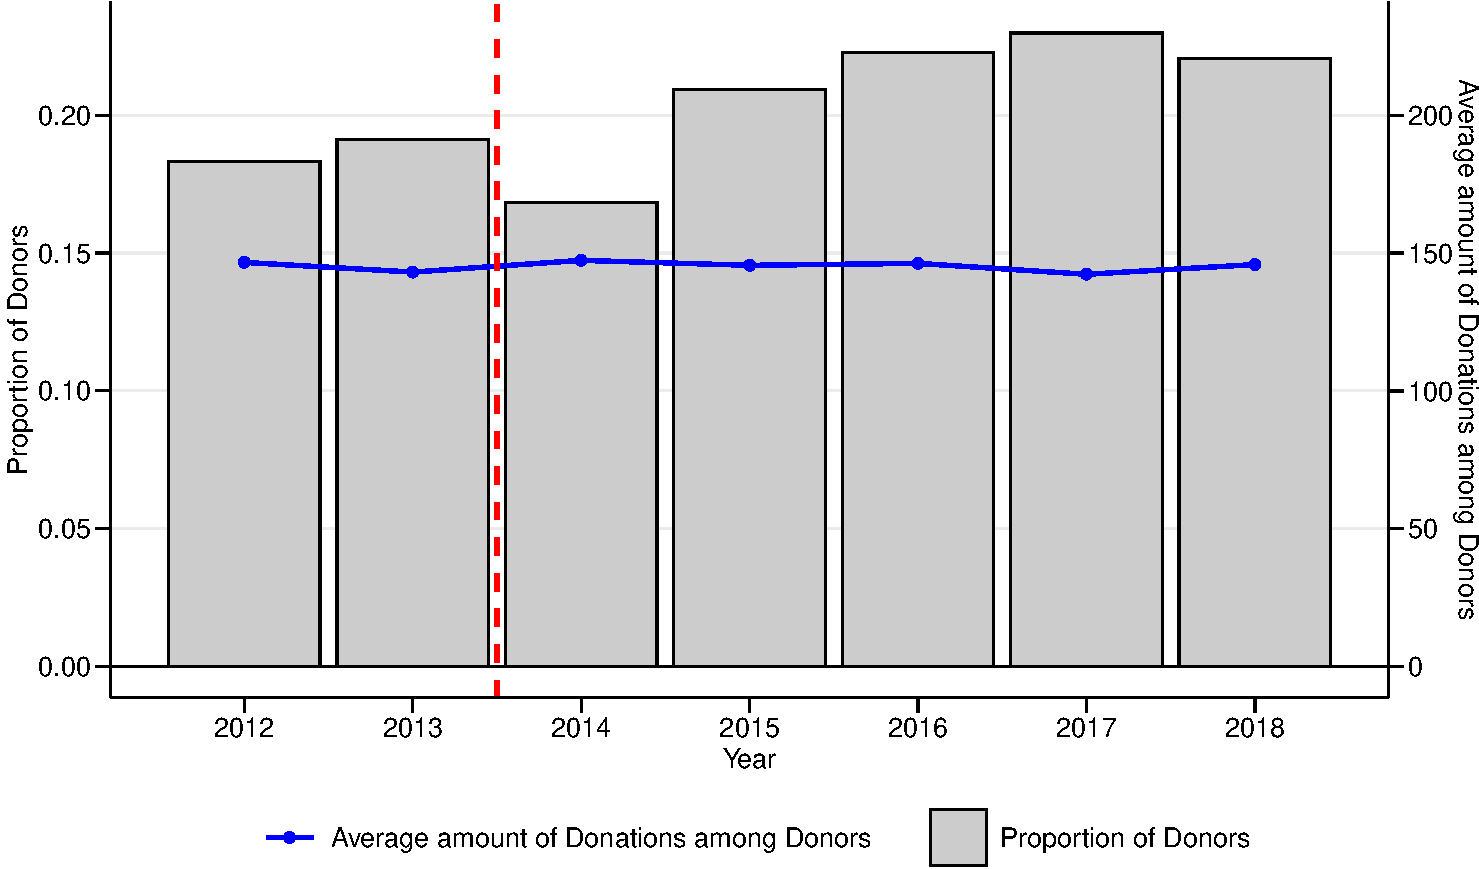
\includegraphics{C:/Users/katoo/Desktop/NASTAB/report/slides_files/figure-beamer/SummaryOutcome-1.pdf}
\caption{Proportion of Donors (bar chart) and Average Donations among
Donors (blue line)}
\end{figure}
\end{frame}

\begin{frame}{Summary Statistics of Covariates}
\protect\hypertarget{summary-statistics-of-covariates}{}
\begin{table}

\caption{\label{tab:kableSummaryCovariate}Summary Statistics of Covariates}
\centering
\fontsize{9}{11}\selectfont
\begin{tabular}[t]{lcccc}
\toprule
 & 2012 & 2013 & 2014 & 2015\\
\midrule
Female & 0.51 & 0.51 & 0.52 & 0.52\\
Age & 38.39 & 39.10 & 39.67 & 40.51\\
Annual Taxable Income & 1699.86 & 1764.04 & 1838.76 & 1872.54\\
\addlinespace[0.3em]
\multicolumn{5}{l}{\textbf{Education}}\\
\hspace{1em}Junior High School Graduate & 0.42 & 0.41 & 0.40 & 0.39\\
\hspace{1em}High School Graduate & 0.30 & 0.30 & 0.31 & 0.31\\
\hspace{1em}University Graduate & 0.28 & 0.28 & 0.29 & 0.30\\
\#.Respondents & 14138 & 13984 & 13787 & 13524\\
\#.Households & 4756 & 4807 & 4819 & 4832\\
\bottomrule
\end{tabular}
\end{table}
\end{frame}

\begin{frame}{Summary Statistics of Covariates (Cont'd)}
\protect\hypertarget{summary-statistics-of-covariates-contd}{}
\begin{table}

\caption{\label{tab:kableSummaryCovariate2}Summary Statistics of Covariates (Continued)}
\centering
\fontsize{9}{11}\selectfont
\begin{tabular}[t]{lccc}
\toprule
 & 2016 & 2017 & 2018\\
\midrule
Female & 0.52 & 0.52 & 0.52\\
Age & 41.07 & 41.89 & 42.55\\
Annual Taxable Income & 1906.91 & 1951.55 & 2039.47\\
\addlinespace[0.3em]
\multicolumn{4}{l}{\textbf{Education}}\\
\hspace{1em}Junior High School Graduate & 0.38 & 0.37 & 0.35\\
\hspace{1em}High School Graduate & 0.31 & 0.31 & 0.31\\
\hspace{1em}University Graduate & 0.31 & 0.33 & 0.34\\
\#.Respondents & 13238 & 12963 & 12795\\
\#.Households & 4790 & 4770 & 4765\\
\bottomrule
\end{tabular}
\end{table}
\end{frame}

\begin{frame}{What is Giving Price?}
\protect\hypertarget{what-is-giving-price}{}
Consider allocation between private consumptions (\(x_i\)) and
charitable giving (\(g_i\)). Let \(y_i\) be pre-tax total income. Then,
the budget constraint is

\[
    x_i + g_i = y_i - T_i(y_i, g_i),
\]

where \(T_i\) is tax amount depending on the pre-tax income and
charitable giving.
\end{frame}

\begin{frame}{Determination of Tax Amount}
\protect\hypertarget{determination-of-tax-amount}{}
Tax deduction reduces taxable income by giving, that is,

\[
    T_i = \tau(y_i - g_i) \cdot (y_i - g_i),
\]

where \(\tau(\cdot)\) is the marginal income tax rate which is
determined by \(y_i - g_i\).

Tax credit reduces tax amount directly, that is,

\[
    T_i = \tau(y_i)\cdot y_i - m g_i,
\]

where \(m \in [0, 1]\) is the tax credit rate.
\end{frame}

\begin{frame}{Derive Giving Price}
\protect\hypertarget{derive-giving-price}{}
Under the tax deduction system, the budget constraint is

\[
    x_i + [1 - \tau(y_i - g_i)]g_i = [1 - \tau(y_i - g_i)] y_i.
\]

Thus, the giving price of tax deduction system is
\(p_i^{d} = 1 - \tau(y_i - g_i)\).

Under the tax credit system, the budget constraint is

\[
    x_i + (1 - m) g_i = [1 - \tau(y_i)] y_i.
\]

Thus, the giving price of tax credit system is \(p_i^c = 1 - m\).
\end{frame}

\begin{frame}{Construct Giving Price}
\protect\hypertarget{construct-giving-price}{}
In the South Korea, the tax policy about charitable giving drastically
changed in 2014.

\begin{itemize}
\tightlist
\item
  tax deduction (before 2014): \(\text{Price}_i = 1 - \tau(y_i - g_i)\)

  \begin{itemize}
  \tightlist
  \item
    the giving price is endogenous because people can manipulate
    \(\tau(y_i - g_i)\) using the charitable giving \(g_i\). Since this
    problem is caused by \emph{last} donations, we use the giving price
    applying to the \emph{first} donations (\textbf{first price}). The
    first price is calculate by \(\tau(y_i)\) where \(y_i\) is the
    annual taxable income reported in the NaSTaB.
  \end{itemize}
\item
  tax credit (after 2014): \(\text{Price}_i = 1 - m\)

  \begin{itemize}
  \tightlist
  \item
    In the South Korea, the tax credit rate determines exogeneity,
    \(m = 0.15\).
  \end{itemize}
\end{itemize}
\end{frame}

\begin{frame}{Income Distribution and Giving Price}
\protect\hypertarget{income-distribution-and-giving-price}{}
\begin{figure}
\centering
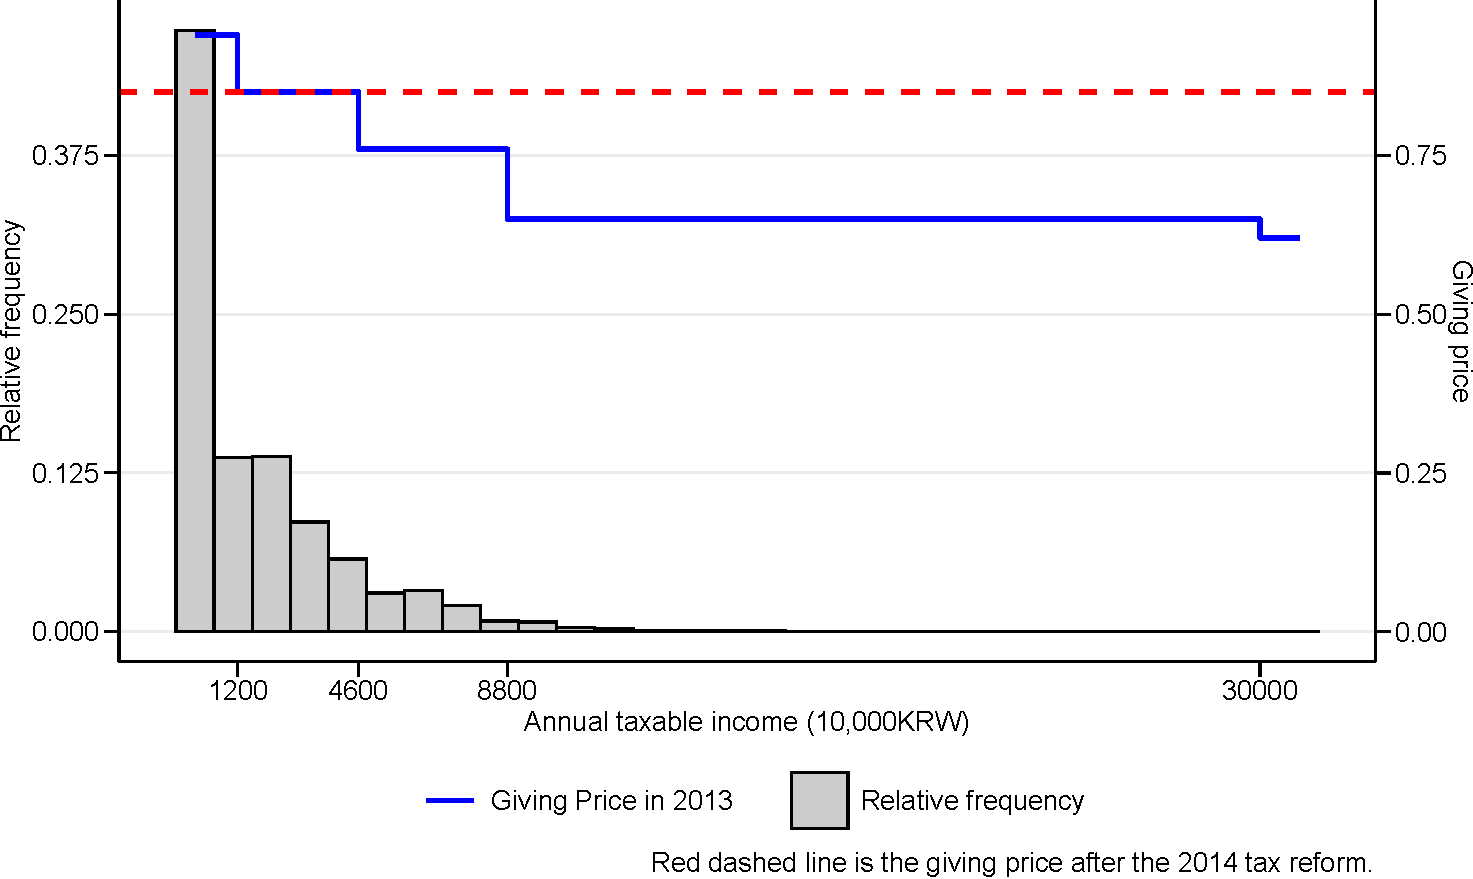
\includegraphics{C:/Users/katoo/Desktop/NASTAB/report/slides_files/figure-beamer/SummaryPriceChange-1.pdf}
\caption{Income Distribution and Giving Price}
\end{figure}
\end{frame}

\hypertarget{price-elasticity}{%
\section{Price Elasticity}\label{price-elasticity}}

\begin{frame}{Baseline Regressions}
\protect\hypertarget{baseline-regressions}{}
Our baseline regression equation is

\[
    \log(\text{Giving}_{ijt}) = 
    \alpha_i + \beta_1 \log(\text{Price}_{ijt}) + \delta X_{ijt} + \lambda_t + \epsilon_{ijt}.
\]

\begin{itemize}
\tightlist
\item
  \(\log(\text{Giving}_{ijt})\) is logarithm of individual \(i\)'s
  charitable giving in year \(t\).
\item
  \(\log(\text{Price}_{ijt})\) is logarithm of individual \(i\)'s giving
  price in year \(t\).
\item
  \(\beta_1\) represents the price elasticity of giving.
\item
  \(\alpha_i\) and \(\lambda_t\) are individual and time fixed effect,
  respectively.
\end{itemize}
\end{frame}

\begin{frame}{Result of Baseline Regressions}
\protect\hypertarget{result-of-baseline-regressions}{}
We found the \textbf{price effect} of giving (1\% price increase leads
to about 1.1\% giving decrease)

\begin{table}

\caption{\label{tab:kableEstimateElasticity}Baseline Regressions}
\centering
\fontsize{9}{11}\selectfont
\begin{tabular}[t]{lccccc}
\toprule
 & (1) & (2) & (3) & (4) & (5)\\
\midrule
ln(giving price) & -1.071*** & -1.071*** & -1.229*** & -1.059*** & -1.062***\\
 & (0.201) & (0.201) & (0.227) & (0.226) & (0.226)\\
Logged Income & Y & Y & Y & Y & Y\\
Age & N & Y & Y & Y & Y\\
Year X Educ & N & N & Y & Y & Y\\
Year X Gender & N & N & N & Y & Y\\
Resident Area & N & N & N & N & Y\\
Obs & 54213 & 54213 & 54211 & 54211 & 54211\\
\bottomrule
\end{tabular}
\end{table}
\end{frame}

\begin{frame}{Robustness Check}
\protect\hypertarget{robustness-check}{}
We addressed the following two potential concerns:

\begin{enumerate}
\tightlist
\item
  Income and donations are determined simultaneously

  \begin{itemize}
  \tightlist
  \item
    This causes both a change of giving price and a change of an amount
    of donations
  \item
    Gruber and Saez (2002) provided that we should use
    \(\log(\text{Price}_{ijt}/\text{Price}_{ij(t-k)})\) as an
    insturment.
  \item
    Following Alumina et al.~(2020), we estimated the model (5) in the
    previous slide, using the panel IV model for \(k = 1, 2, 3, 4\).
  \end{itemize}
\item
  The effect of presidential transition on donations

  \begin{itemize}
  \tightlist
  \item
    The presidential transition is one of our major ommited factor to
    affect both political trust and charitable giving.
  \item
    To shed light on this concern, we used data in 2013 and 2014
    (President was Park Geun-hye in both years), and estimated the model
    (5) in the previous slide, using the fixed effect model and the
    panel IV model for \(k = 1, 2, 3, 4\).
  \end{itemize}
\end{enumerate}
\end{frame}

\begin{frame}{Result of Robustness Check 1}
\protect\hypertarget{result-of-robustness-check-1}{}
We obtained similar value of price elasticity to baseline results (1\%
price increase leads to about 1.1\% giving decrease)

\begin{table}

\caption{\label{tab:kableRobust1EstimateElasticity}Panel IV Regressions}
\centering
\begin{tabular}[t]{lcccc}
\toprule
 & k = 1 & k = 2 & k = 3 & k = 4\\
\midrule
ln(giving price) & -1.160** & -1.088*** & -1.138*** & -0.941***\\
 & (0.473) & (0.411) & (0.368) & (0.336)\\
F-stat of IV & 10671.085 & 11547.015 & 11742.698 & 9585.022\\
Obs & 51982 & 49707 & 46878 & 43651\\
\bottomrule
\end{tabular}
\end{table}
\end{frame}

\begin{frame}{Result of Robustness Check 2}
\protect\hypertarget{result-of-robustness-check-2}{}
We obtained \textbf{stonger} price effect than baseline (1\% price
increase leads to about 1.2 \textasciitilde{} 1.6\% giving decrease)

\begin{table}

\caption{\label{tab:kableRobust2EstimateElasticity}Results with data in 2013 and 2014}
\centering
\fontsize{9}{11}\selectfont
\begin{tabular}[t]{lccccc}
\toprule
\multicolumn{1}{c}{ } & \multicolumn{1}{c}{FE} & \multicolumn{4}{c}{Panel IV with FE} \\
\cmidrule(l{3pt}r{3pt}){2-2} \cmidrule(l{3pt}r{3pt}){3-6}
 &  & k = 1 & k = 2 & k = 3 & k = 4\\
\midrule
ln(giving price) & -1.466*** & -1.497*** & -1.628*** & -1.207*** & -1.331***\\
 & (0.327) & (0.355) & (0.375) & (0.381) & (0.395)\\
F-stat of IV &  & 7374.556 & 4635.809 & 5157.662 & 5207.029\\
Obs & 15134 & 13870 & 13095 & 12564 & 11774\\
\bottomrule
\end{tabular}
\end{table}
\end{frame}

\hypertarget{political-trust-and-price-elasticity}{%
\section{Political Trust and Price
Elasticity}\label{political-trust-and-price-elasticity}}

\begin{frame}{Estimation of Trust Index}
\protect\hypertarget{estimation-of-trust-index}{}
The trust for politicans is time-varying variable because it depends on
governments' policies. We make time-invarying trust index using the
fixed effect model.

\[
    \text{Trust}_{ijt} = \text{Trustid}_{ij} + c_j \cdot \lambda_t + \lambda_t + \epsilon_{ijt}.
\]

\begin{itemize}
\tightlist
\item
  \(\text{Trust}_{ijt}\): trust for politicians (5-Likert scale)
\item
  \(\text{Trustid}_i\): individual fixed effect (\textbf{Trust index})
\item
  \(c_j \cdot \lambda_t\) captures local governments' policies effect
\item
  \(\lambda_t\) captures the central government policies effect
\end{itemize}
\end{frame}

\begin{frame}{Histrogram of Trust Index}
\protect\hypertarget{histrogram-of-trust-index}{}
\begin{figure}
\centering
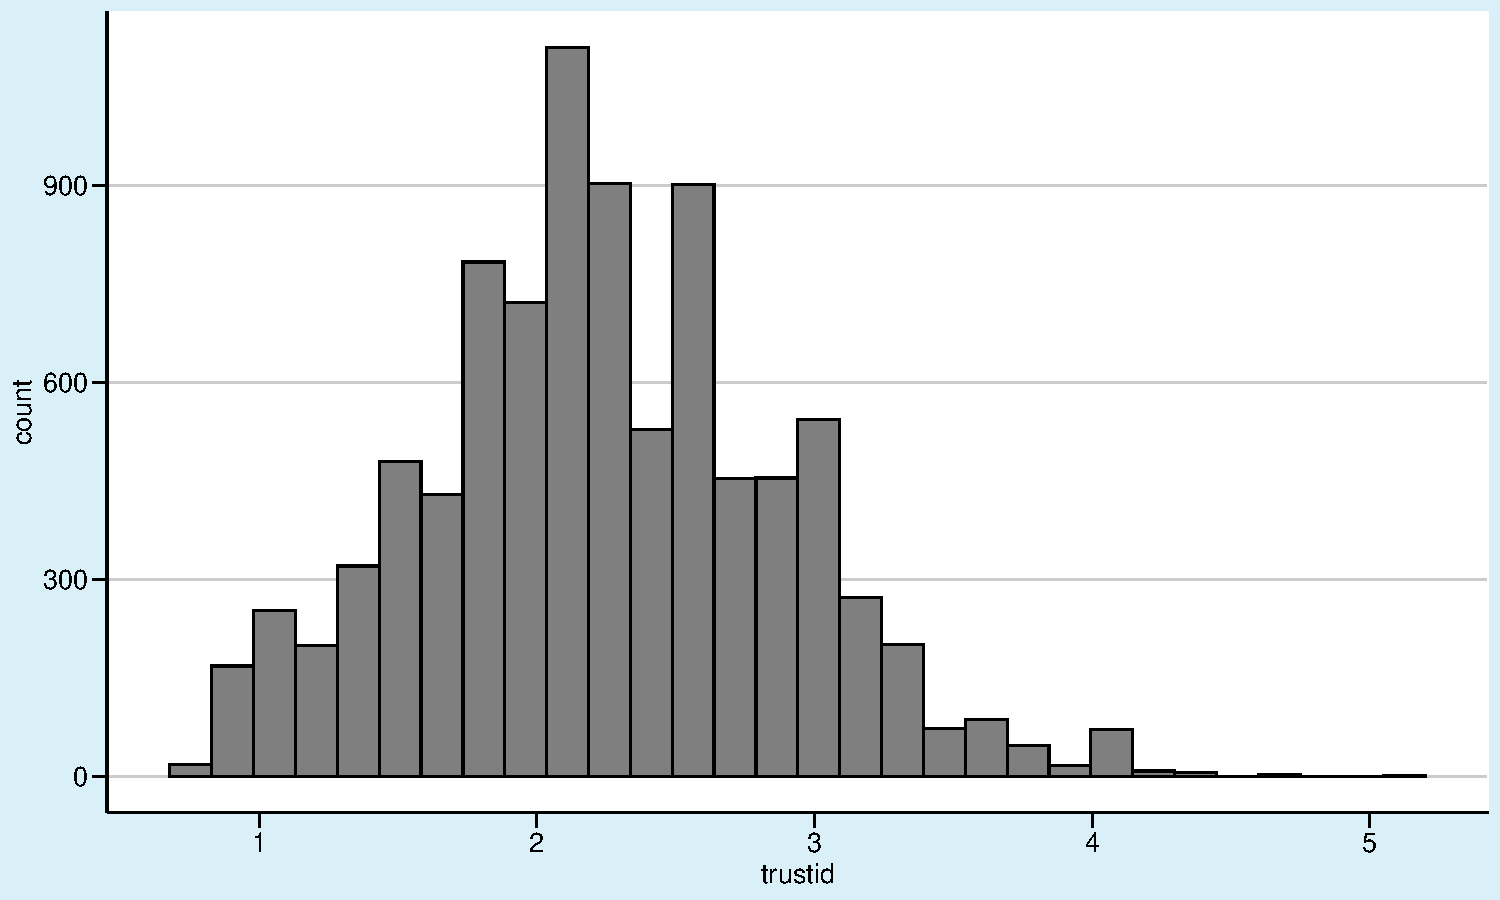
\includegraphics{C:/Users/katoo/Desktop/NASTAB/report/slides_files/figure-beamer/HistogramTrustid-1.pdf}
\caption{Histogram of Trust Index}
\end{figure}
\end{frame}

\begin{frame}{Relationship with Donations and Covariates}
\protect\hypertarget{relationship-with-donations-and-covariates}{}
\begin{itemize}
\tightlist
\item
  We made a scatter plot b/w individual average donations and trust
  index

  \begin{itemize}
  \tightlist
  \item
    No linear relationship
  \end{itemize}
\item
  We tested difference in mean of individual average donations b/w among
  those whose trust index above and below threshold

  \begin{itemize}
  \tightlist
  \item
    The difference in mean is statistically siginificant at 5\% level if
    threshold is \(\{2.9, 3.0, 3.1, 3.2, 3.3, 3.4, 3.5\}\).
  \end{itemize}
\item
  We regressed trust index on covariates, using data in 2018

  \begin{itemize}
  \tightlist
  \item
    trust among females \textless{} trust among males
  \item
    the positive correlation between income and trust index
  \item
    trust index is concave in age
  \item
    Those having extreme political views have a distrust of politicians
    rather than those having moderate political views.
  \end{itemize}
\end{itemize}
\end{frame}

\begin{frame}{Relationship b/w Donations and Trust Index}
\protect\hypertarget{relationship-bw-donations-and-trust-index}{}
\begin{figure}
\centering
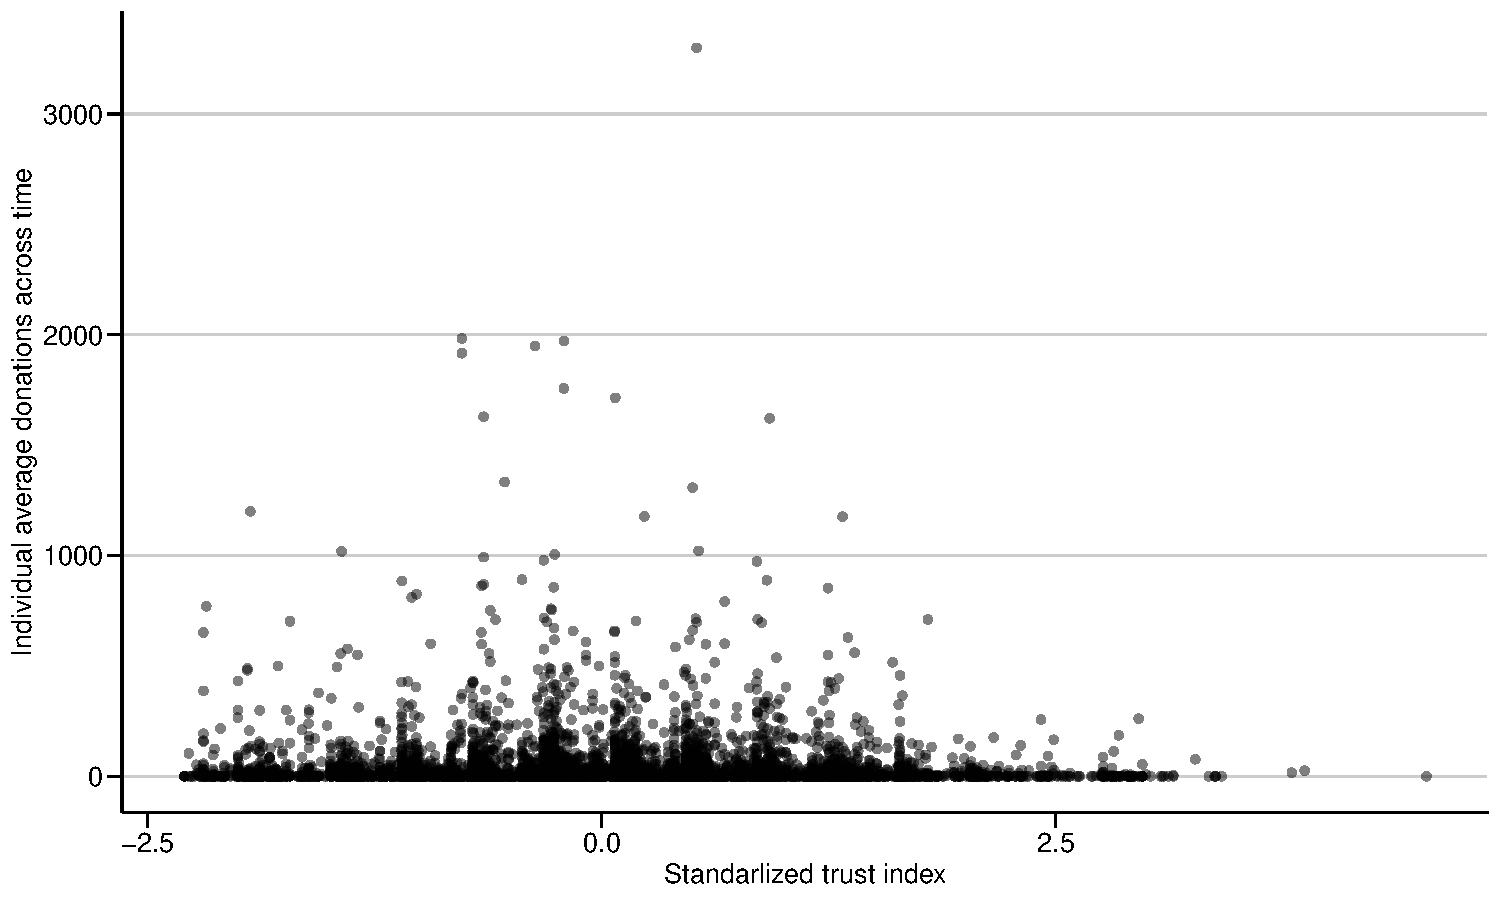
\includegraphics{C:/Users/katoo/Desktop/NASTAB/report/slides_files/figure-beamer/ScatterTrusidDonations-1.pdf}
\caption{Scatter Plot between Donations and Trust Index}
\end{figure}
\end{frame}

\begin{frame}{Difference in Mean b/w Two Trust Groups}
\protect\hypertarget{difference-in-mean-bw-two-trust-groups}{}
\begin{figure}
\centering
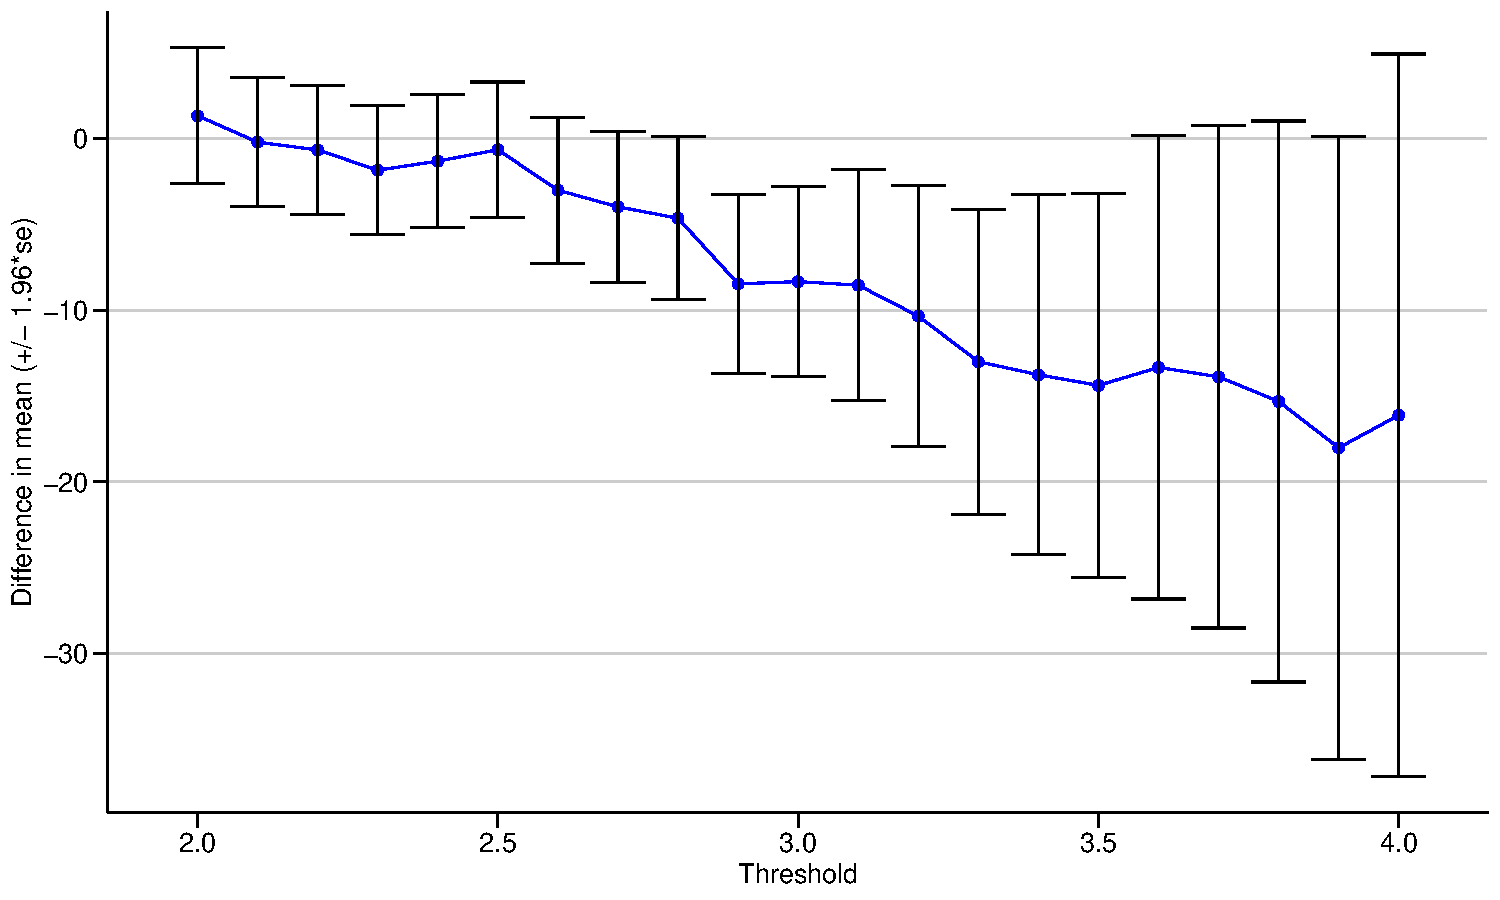
\includegraphics{C:/Users/katoo/Desktop/NASTAB/report/slides_files/figure-beamer/PlotDiffDonationsbwTrustGroup-1.pdf}
\caption{Difference in Mean between Trust Group above and below
Threshold}
\end{figure}
\end{frame}

\begin{frame}{Regression of Trust Index on Covariates}
\protect\hypertarget{regression-of-trust-index-on-covariates}{}
\begin{table}

\caption{\label{tab:kableRegTrustidOnCovariate}Regression of Standarized Trust Index (Year = 2018)}
\centering
\begin{tabular}[t]{lcc}
\toprule
Variables & Coefficients & S.E.\\
\midrule
Female & 0.036** & (0.015)\\
Logarithm of income & 0.529* & (0.281)\\
Age & -0.014*** & (0.003)\\
squared age/100 & 0.014*** & (0.002)\\
High school graduate & 0.018 & (0.023)\\
University graduate & 0.006 & (0.024)\\
Extreme right wing & -0.143*** & (0.054)\\
Right wing & -0.023 & (0.018)\\
Left wing & -0.050*** & (0.018)\\
Extreme left wing & -0.424*** & (0.029)\\
Obs & 7697 & \\
\bottomrule
\end{tabular}
\end{table}
\end{frame}

\begin{frame}{Subgroup Regressions}
\protect\hypertarget{subgroup-regressions}{}
To see the heterogenous price elasticity by political trust, We
estimated the baseline regression model (5) (see Table
\ref{tab:kableEstimateElasticity}), using sample grouped by the trust
index.

\begin{itemize}
\tightlist
\item
  Lowest: 0 \textasciitilde{} 20\% quantile of trust index
\item
  Lower: 20 \textasciitilde{} 40\% quantile of trust index
\item
  Neutral: 40 \textasciitilde{} 60\% quantile of trust index
\item
  Higher: 60 \textasciitilde{} 80\% quantile of trust index
\item
  Highest: 80 \textasciitilde{} 100\% quantile of trust index
\end{itemize}

Covariates are the logarithm of income, age, interactions b/w year and
education, interactions b/w year and gender, and living are dummy into
covariates.
\end{frame}

\begin{frame}{Results of Subgroup Regressions}
\protect\hypertarget{results-of-subgroup-regressions}{}
We cound \textbf{NOT} find the price effect for respondents whose trust
is very low.

\begin{table}

\caption{\label{tab:kableEstimateElasticityByTrustGroup}Subgroup Regressions}
\centering
\fontsize{9}{11}\selectfont
\begin{tabular}[t]{lccccc}
\toprule
 & Lowest & Lower & Neutral & Higher & Highest\\
\midrule
ln(giving price) & -0.675 & -0.460 & -1.667*** & -1.186** & -1.338**\\
 & (0.558) & (0.459) & (0.481) & (0.531) & (0.552)\\
Obs & 10239 & 10358 & 10432 & 10303 & 9969\\
\bottomrule
\end{tabular}
\end{table}
\end{frame}

\begin{frame}{Regression on Interaction Term}
\protect\hypertarget{regression-on-interaction-term}{}
To check whether price elasticity is statistically siginificant
different among five trust groups, we estimated the baseline regression
model (5) including interation term between five trust groups and giving
price.

\begin{align*}
    \log(\text{Giving}_{ijt}) 
    =& \alpha_i + \beta_1 \log(\text{Price}_{ijt}) \\
    &+ \sum_g \beta_g \log(\text{Price}_{ijt}) \cdot \text{TrustGroup}_{ijg}  \\
    &+ \delta X_{ijt} + \lambda_t + \epsilon_{ijt}.
\end{align*}

\begin{itemize}
\tightlist
\item
  \(\text{TrustGroup}_{ijg}\): taking 1 if individual \(i\) living in
  \(j\) belongs to the trust group \(g\).
\item
  \(g \in \{ \text{Lowest}, \text{Lower}, \text{Higher}, \text{Highest} \}\).
\end{itemize}
\end{frame}

\begin{frame}{Regression Result on Interation Term}
\protect\hypertarget{regression-result-on-interation-term}{}
There is statistically siginificant difference on price elasticity
between the lowest group and the nuetral group.

\begin{table}

\caption{\label{tab:kableEstimateInteractionByTrustGroup}Heterogenous Price Elasticity}
\centering
\begin{tabular}[t]{lcc}
\toprule
 & Coefficients & S.E.\\
\midrule
ln(giving price) & -1.646*** & (0.393)\\
X Lowest Trust & 1.291** & (0.531)\\
X Lower Trust & 0.833 & (0.514)\\
X Higher Trust & 0.275 & (0.541)\\
X Highest Trust & 0.372 & (0.531)\\
Obs & 51301 & \\
\bottomrule
\end{tabular}
\end{table}
\end{frame}

\hypertarget{conclusions}{%
\section{Conclusions}\label{conclusions}}

\begin{frame}{Conclusions}
\protect\hypertarget{conclusions-1}{}
\end{frame}

\end{document}
